\section{Experimental evaluation}\label{sec:experiment}
In this section, an experimental evaluation over three real-life event logs is reported.


\subsection{Re-sampling and test setup}
In order to obtain training data, time series are obtained by specifying a number of intervals (i.e. time steps in the DF time series) using either equitemporal or equisize aggregation a described in Section \ref{sec:preliminaries}.
Time series algorithms are parametric and sensitive to sample size requirements \cite{hanke2001business}.
Depending on the number of parameters a model uses, a minimum size of at least 50 steps is not uncommon, although typically model performance should be monitored at a varying number of steps.
In the experimental evaluation, the event logs are divided into 100 time steps with a varying share of training and test steps: $h=25$ meaning all test sets contain 25 intervals, and the training sets are varied from $ts=25$ to $ts=75$ steps, meaning the forecasts progressively target the prediction of steps 25-50 (the second quarter of intervals) over to 75-100 (the last quarter of intervals).
This allows to both inspect the difference in results when only few data points are used, and whether there is a difference forecasting data points in the middle or towards the end of the available event data.
Resampling is applied based on a 10-fold cross-validation constructed following a rolling window approach for all horizon values $h\in[1,25]$ where a recursive strategy is used to iteratively obtain $\hat{y}_{t+h|T_{t+h-1}}$ with $(y_1,\dots,y_{T},\dots,\hat{y}_{t+h-1})$ \cite{weigend2018time}.
10 training sets are hence constructed for each training set length $ts$ and exist from $(y_1,\dots,y_{T-h-f})$ and the test sets from $(y_{T-h-f+1},\dots,y_{T-f})$ with $f\in[0,9]$ the fold index \cite{bergmeir2012use}.
While direct strategies with a separate model for every value of $h$ can be used as well and avoid the accumulation of error, they do not take into account statistical dependencies for subsequent predictions.

Three widely-used event logs are used: the 2012 BPI challenge log\footnote{\url{https://doi.org/10.4121/uuid:3926db30-f712-4394-aebc-75976070e91f}}, the Sepsis cases event log\footnote{\url{https://doi.org/10.4121/uuid:915d2bfb-7e84-49ad-a286-dc35f063a460}}, and the Road Traffic Fine Management Process log\footnote{\url{https://doi.org/10.4121/uuid:270fd440-1057-4fb9-89a9-b699b47990f5}} (RTFMP) event log.
Each of these logs has a diverse set of characteristics in terms of case and activity volume, as well as average trace length as can be seen in Table \ref{tab:eventlogs}.
\begin{table}[htbp]
  \centering
    \begin{tabular}{lrrr}
    \toprule
    \textbf{Event log} & \multicolumn{1}{l}{\textbf{\# cases}} & \multicolumn{1}{l}{\textbf{\# activities}} & \multicolumn{1}{l}{\textbf{Average trace length}} \\
    \midrule
    \textbf{BPI 12} & 13,087 & 36    & 20.020 \\
    \textbf{Sepsis} & 1,050 & 16    & 14.490 \\
    \textbf{RTFMP} & 150,370 & 11    & 3.734 \\
    \bottomrule
    \end{tabular}%
  \caption{Overview of the characteristics of the event logs used in the experimental evaluation.}
  \label{tab:eventlogs}%
\end{table}%

An example of applying the equisize or equitemporal aggregation to the Sepsis event log with 100 intervals results in the DF time series of Figure \ref{fig:sepsists} where the DF occurrences of the most frequently occurring activity pair is included.
For the equisized aggregation the number of DFs is indeed relatively stable over the log's timeline where for the equitemporal aggregation a noticeable decline of DF pairs is visible towards the end of the series.
This phenomenon is typical in event logs, as processes typically have particular endpoint activities, but can also be due to the unequal distribution of events over the event log's time line.
If the level of occurrences of the DF pair is low and close to 0, the series might be too unsuitable for analysis with white noise series analysis techniques that assume stationarity.
Ideally, every time series is tested using a stationarity test such as the Dickey-Fuller unit root test \cite{leybourne1995testing} and an appropriate lag order is established for differencing. 
Furthermore for each algorithm, especially ARIMA-based models, (partial) auto-correlation could establish the ideal $p$ and $q$ parameters.
However, for the sake of simplicity and to avoid tedious solutions where each activity pair has to have different parameters, various values are used for $p$, $d$, and $q$ and applied to all DF pairs where only the best-performing are reported below for comparison with the other time series techniques.

% \begin{figure}[tb]
% 	\centering
% 	\subfigure[Most common DF - equisize]{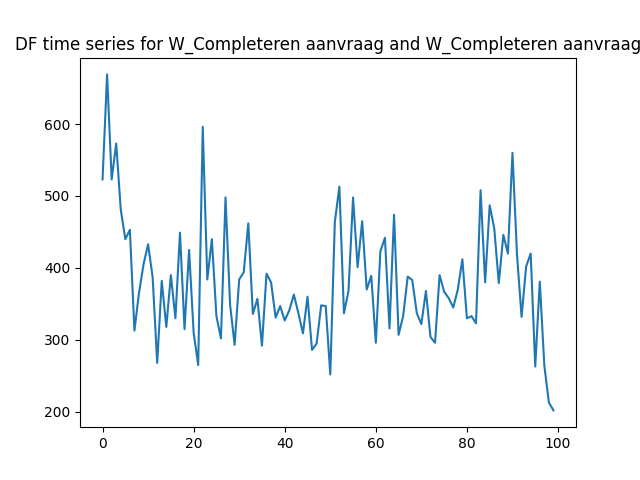
\includegraphics[width=0.49\textwidth]{./img/bpi12_1.png}}
% 	\subfigure[Most common DF - equitemp]{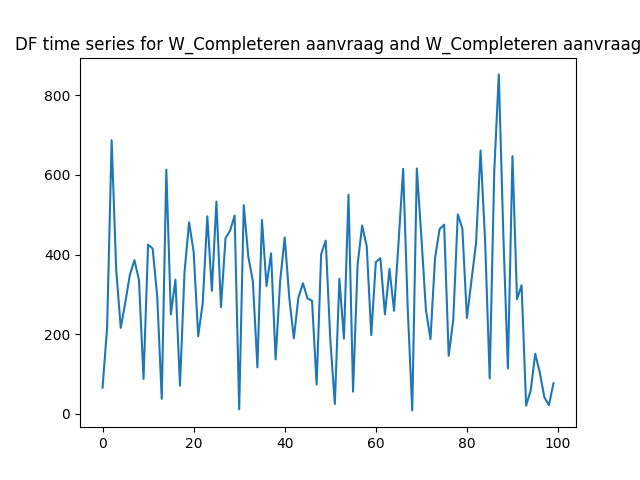
\includegraphics[width=0.49\textwidth]{./img/bpi12_1_t.png}}
% 	\caption{BPI 12}
% 	\label{fig:bpi12ts}
% \end{figure}

\begin{figure}[tb]
	\centering
	\subfigure[Most common DF - equisize]{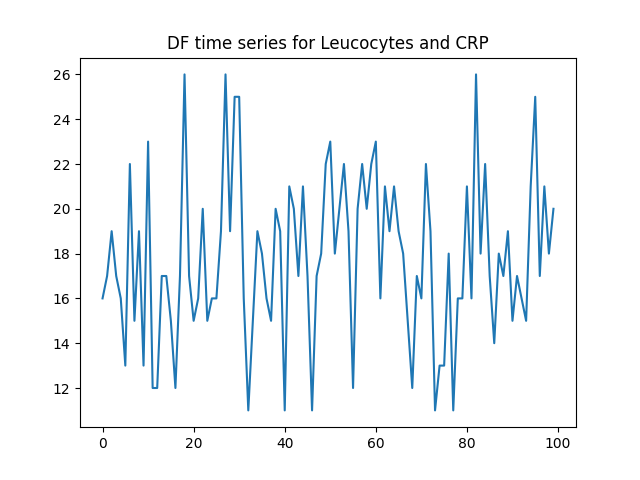
\includegraphics[width=0.39\textwidth]{./img/sepsis_1.png}}
	\subfigure[Most common DF - equitemp]{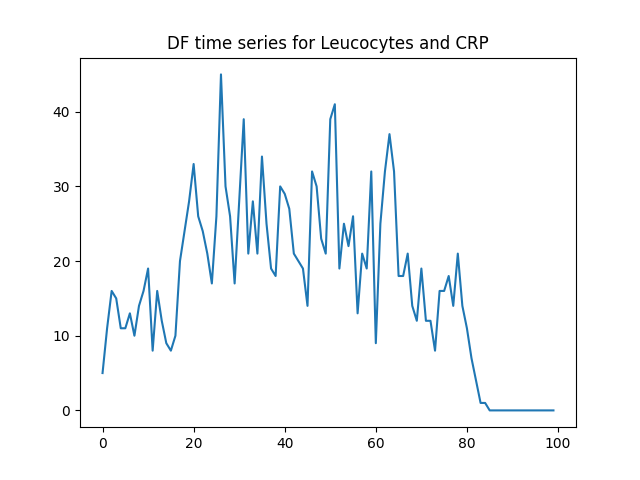
\includegraphics[width=0.39\textwidth]{./img/sepsis_1_t.png}}
	\caption{Sepsis}
	\label{fig:sepsists}
\end{figure}

% \begin{figure}[tb]
% 	\centering
% 	\subfigure[Most common DF - equisize]{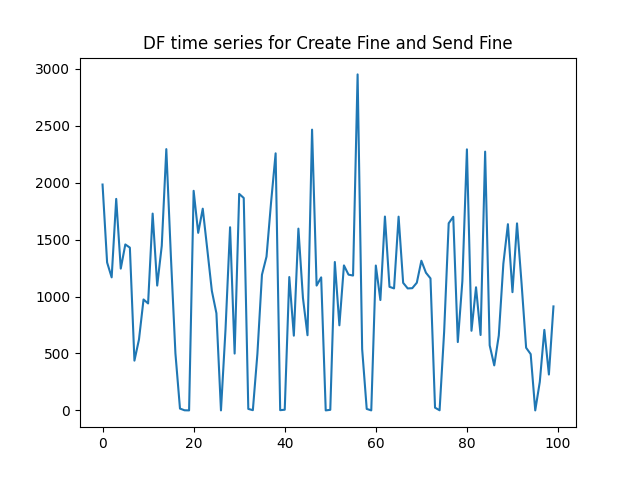
\includegraphics[width=0.49\textwidth]{./img/rtfmp_1.png}}
% 	\subfigure[Most common DF - equitemp]{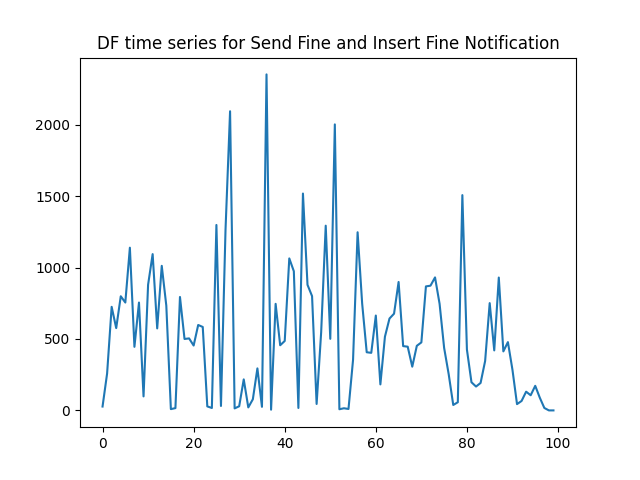
\includegraphics[width=0.49\textwidth]{./img/rtfmp_1_t.png}}
% 	\caption{RTFMP}
% 	\label{fig:rtfmpts}
% \end{figure}

Given that we want to evaluate the capability of the approach to accurately predict the evolution of the process model, the combination of all DF predictions to obtain a global DFG prediction is considered.
The following two criteria are used:
\begin{itemize}
	\item \textbf{Cosine distance:} measures the distance between two vectors and is often used to compare graph distance. This metric is used to compare the DFG's edge weight matrices between the actual and predicted number of DF relations.
	\item \textbf{Entropic relevance:} a measure for stochastic conformance checking computed as the average number of bits required to compress each of the log’s traces based on the structure and information about relative likelihoods provided by the model \cite{DBLP:conf/icpm/PolyvyanyyMG20}.
\end{itemize}
These criteria balance a predictive and structural evaluation of the algorithms and report on both the numeric performance common in a forecasting setting as well as their appropriateness in terms of reproducing a structurally usable process model which allows for the observed process behavior.
In both cases a lower score is better.
The entropic relevance also allows to compare the adequacy the forecasted DFGs with the actual DFGs.

\subsection{Results}
All pre-processing was done in Python with a combination of \emph{pm4py}\footnote{\url{https://pm4py.fit.fraunhofer.de}} and the \emph{statsmodels} package \cite{seabold2010statsmodels}. 
The code is available %TODO here.

The results are displayed in Figures \ref{fig:bpi12_equisize} to \ref{fig:rtfmp_equitemp}. - STILL NEED TO REDUCE THESE FIGURES. ANY INPUT WOULD BE HELPFUL (definitely no need to keep all ARIMAs I think). 

NOTE THAT ALL FIGURES ARE AVAILABLE IN Results PMF 08-03.zip

Observations:
\begin{itemize}
    \item Regardless of the aggregation type, only using 25-35 training points to forecast 25 test points creates very unstable results for all datasets and forecasting techniques both in terms of cosine distance and entropic relevance. Especially autoregressive models (both AR and ARIMA) from a higher order (2,4) suffer from very high cosine distances when few training points are used. 
    This is potentially due to the inclusion of more distant observations in the prediction.
    \item Once a level of stability is present in the results, the difference between forecasting techniques is lower in terms of the cosine distance although GARCH and AR models still perform worse. 
    \item In terms of entropic relevance, the actual DFGs do have better scores except for the BPI 12 log where GARCH even outperforms the actual DFG. In general, GARCH scores best in terms of entropic relevance while the other models perform similar to the naive model. ARIMA models perform worst overall.
    \item For the equitemporal aggregation this difference of the actual with the forecasts is less pronounced and the difference among the forecasts is minimal as well. 
    The entropic relevance is also significantly higher for the equitemporal aggregation.
\end{itemize}

Implications:
\begin{itemize}
    \item The entropic relevance learns us that the forecasting techniques are capable of obtaining similar results capturing as much of the process behavior as the actual DFGs generated by the process.
    \item The forecasting techniques used have little impact, meaning that even a naive forecast can produce good results, although GARCH models perform better, possibly due to their capturing a varying level of variance over time which seems especially suitable for DF relations which do not necessarily are generated by a white noise process. Note, however, that the confidence intervals have not yet been investigated.
    \item The results show that there is a need to have at least observed close to half of the process' events before reasonably stable predictions can be made.
    \item An equitemporal aggregation results in worse forecasts. This is potentially due to the inconsitent number of DF occurrences present, compared to the equisize aggregation which is stable and hence approaches a white noise process.
\end{itemize}

%TODO: select which figures to include here, as these take up 3 pages:
\begin{figure}
    \centering
    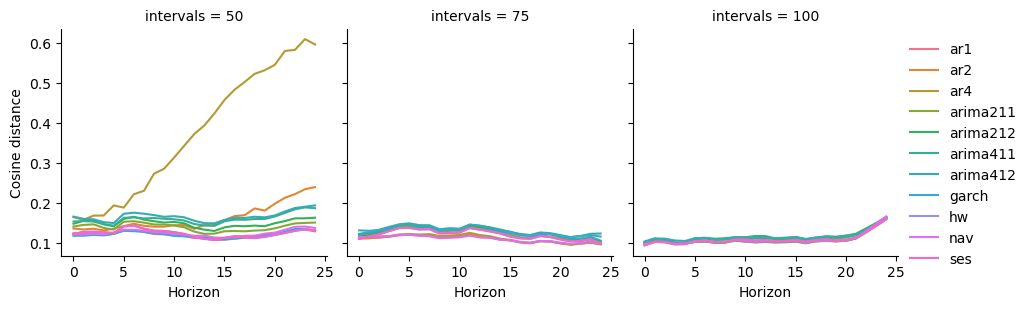
\includegraphics[width=\textwidth]{img/bpi12_cosine_equisize.png}
    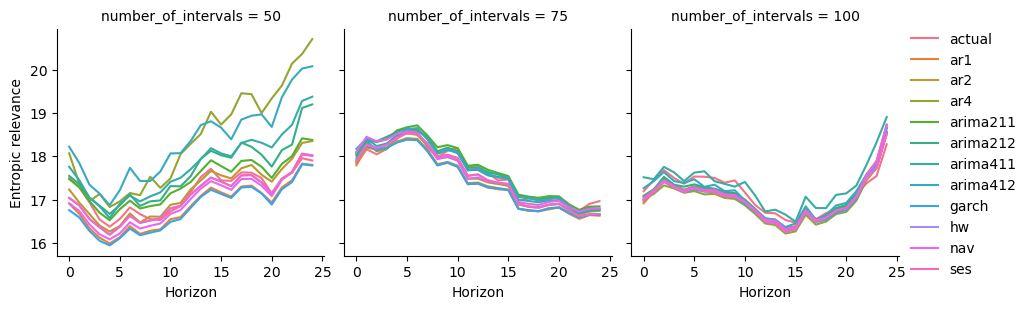
\includegraphics[width=\textwidth]{img/bpi12_entropic_equisize.png}
    \caption{Results for equi-size aggregation for the BPI12 event log.}
    \label{fig:bpi12_equisize}
\end{figure}

\begin{figure}
    \centering
    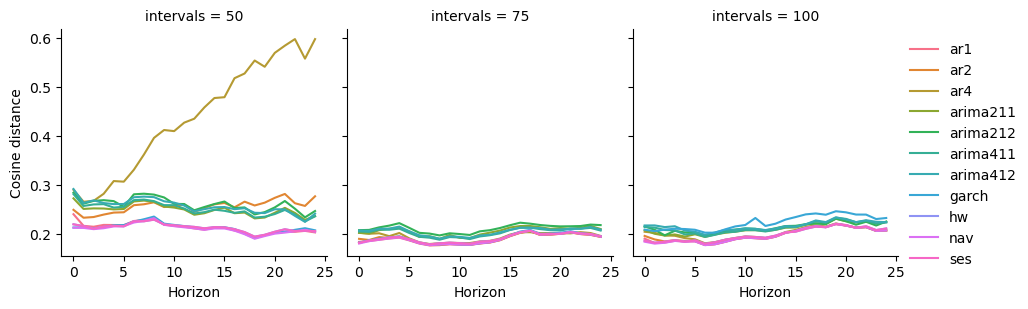
\includegraphics[width=\textwidth]{img/sepsis_cosine_equisize.png}
    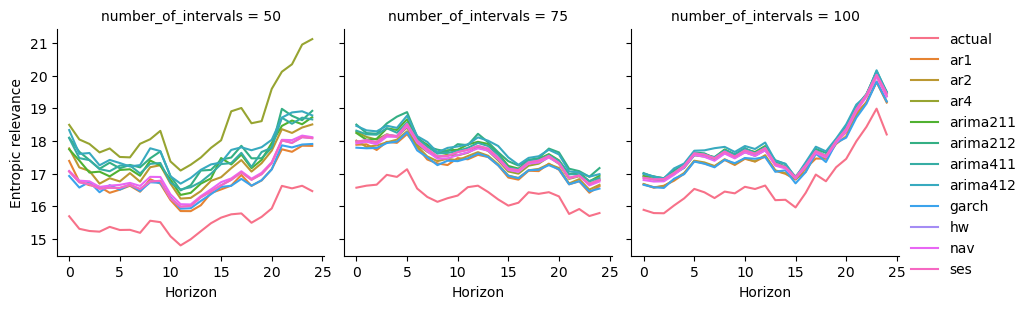
\includegraphics[width=\textwidth]{img/sepsis_entropic_equisize.png}
    \caption{Results for equi-size aggregation for the sepsis event log.}
    \label{fig:sepsis_equisize}
\end{figure}

\begin{figure}
    \centering
    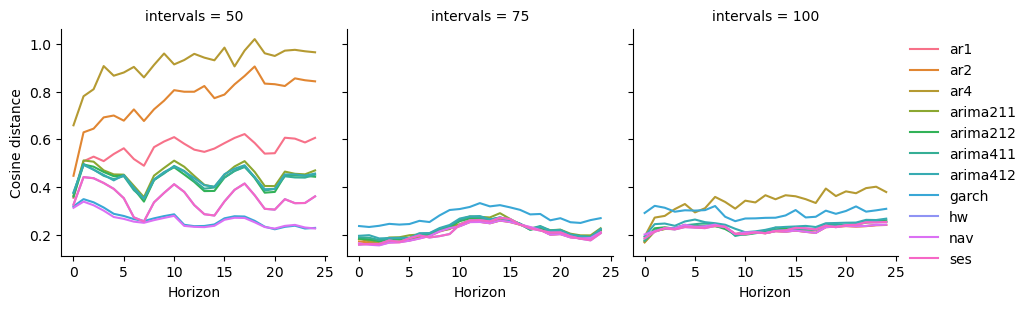
\includegraphics[width=\textwidth]{img/rtfmp_cosine_equisize.png}
    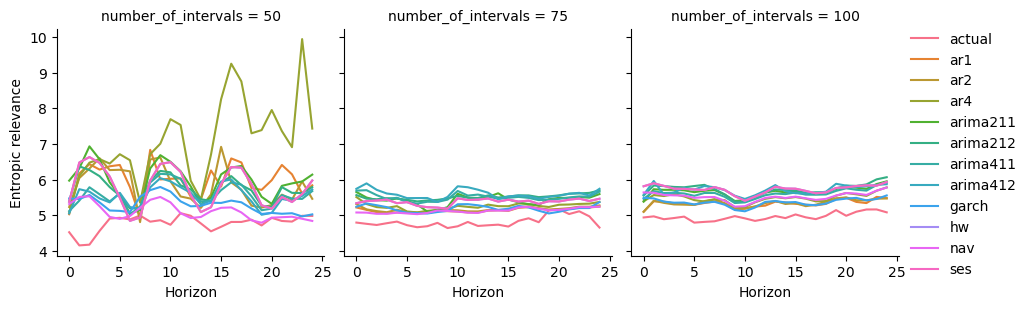
\includegraphics[width=\textwidth]{img/rtfmp_entropic_equisize.png}
    \caption{Results for equi-size aggregation for the RTFMP event log.}
    \label{fig:rtfmp_equisize}
\end{figure}

\begin{figure}
    \centering
    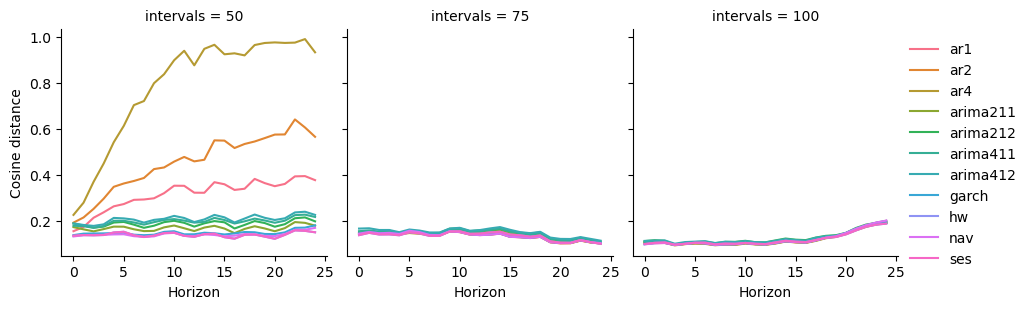
\includegraphics[width=\textwidth]{img/bpi12_cosine_equitemp.png}
    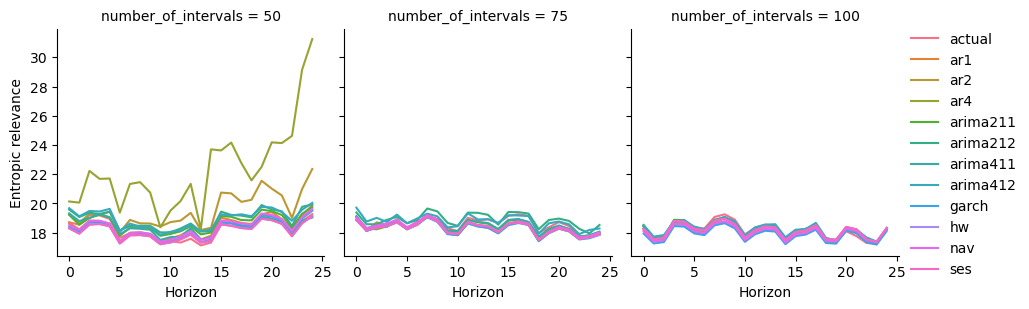
\includegraphics[width=\textwidth]{img/bpi12_entropic_equitemp.png}
    \caption{Results for equi-temporal aggregation for the BPI12 event log.}
    \label{fig:bpi12_equitemp}
\end{figure}

\begin{figure}
    \centering
    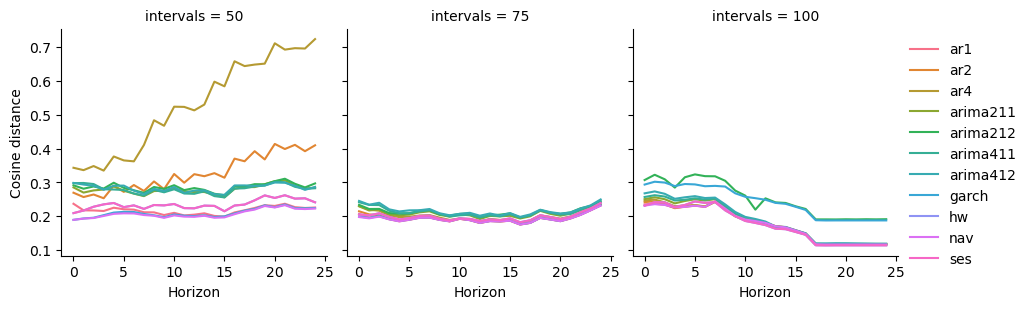
\includegraphics[width=\textwidth]{img/sepsis_cosine_equitemp.png}
    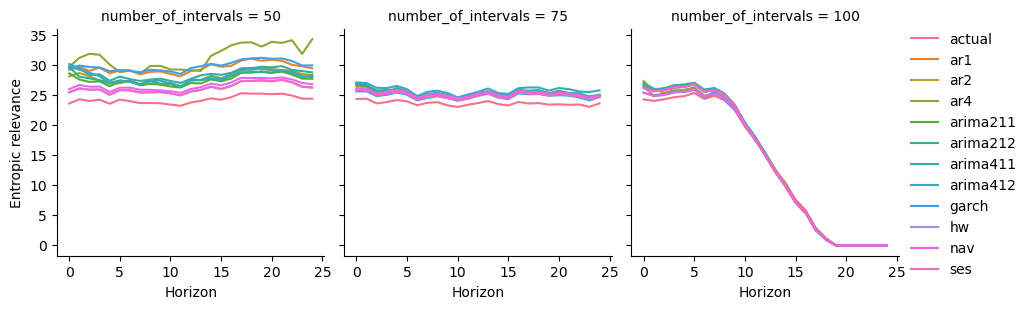
\includegraphics[width=\textwidth]{img/sepsis_entropic_equitemp.png}
    \caption{Results for equi-temporal aggregation for the sepsis event log.}
    \label{fig:sepsis_equitemp}
\end{figure}

\begin{figure}
    \centering
    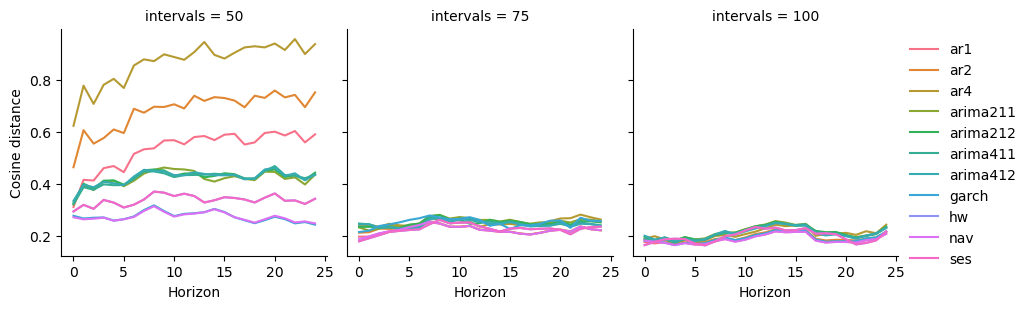
\includegraphics[width=\textwidth]{img/rtfmp_cosine_equitemp.png}
    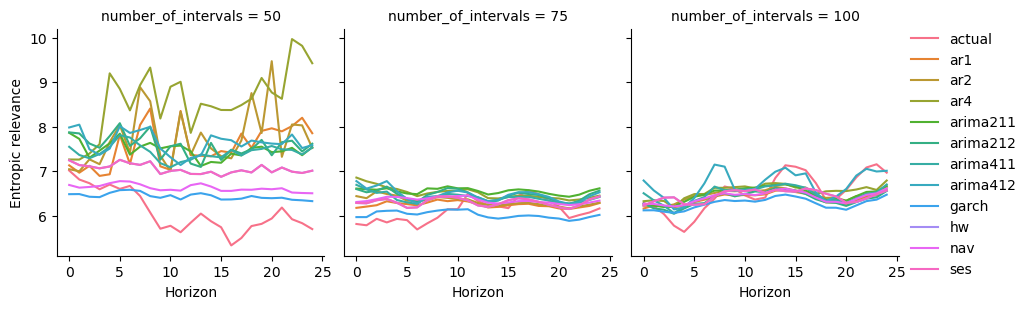
\includegraphics[width=\textwidth]{img/rtfmp_entropic_equitemp.png}
    \caption{Results for equi-temporal aggregation for the RTFMP event log.}
    \label{fig:rtfmp_equitemp}
\end{figure}


